\chapter{Estimation of Active Sources}\label{ch:estimation_k}
In this chapter the issue of unknown number of active sources $k$ is considered. 
The aim is to investigate the possibility of identifying an estimation of a non-active source signal from $\hat{\textbf{X}}_{\text{main}}$ when the true $k$ is not provided to the main algorithm. 
Instead of providing the true $k$ one let $k = N$.
As such one ask the main algorithm for $N$ active source signals, but there are only $k < N$ active source signal. 
At first the possibilities are investigated on synthetic data set, cf. section \ref{sec:dataset} and afterwards the real EEG data set.   

\section{Empirical Test on Synthetic Data}
Figure \ref{fig:ktest1} visualize the estimate $\hat{\mathbf{X}}_{\text{main}}$ from a stochastic data set specified by $M = N = 8$, $k = 4$ and $L = 1000$. 
As seen in section \ref{sec:testMsbl_stoch} the case of $M = N$ should be solved almost exact by the M-SBL algorithm with true $\mathbf{A}$. 
From the figure it is seen that the estimates of the zero rows have amplitudes close to zero.
This distinguishes them from the remaining estimates which are seen to be almost exact. 
Due to the estimates of the zero rows being this close to zero they do not affect the MSE. 
Thus, the MSE do not indicate flaws within the estimate. 
Furthermore, it is seen that the estimates of the zero rows form a scaled copy of one of the exact estimates. 
These observations indicate a potential for distinguishing the estimates of zero rows and hence determine $k$.     
\begin{figure}[H]
    \centering
	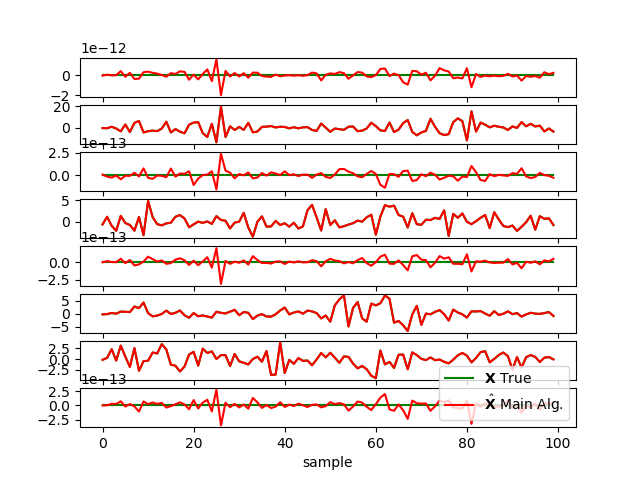
\includegraphics[scale=0.5]{figures/ch_estimate/k_test1.png}
	\caption{Each plot shows one row of the estimate $\hat{\mathbf{X}}_{\text{main}}$ using true $\mathbf{A}$, compared to the corresponding true row in $\mathbf{X}$. The MSE is $1.196E-29$. Only samples in the interval $[0,100]$ are plotted.}
	\label{fig:ktest1}
\end{figure}
\noindent
Consider now the desired case where $M < N$.
Figure \ref{fig:ktest3} visualize the estimate $\hat{\mathbf{X}}_{\text{main}}$ from a stochastic data set specified by $M = 6$, $N = 8$, $k = 4$ and $L = 1000$.
From figure \ref{fig:ktest3} it is seen that the estimates of the zero rows is not as close to zero as in figure \ref{fig:ktest1}. 
Thus, this can not be used as the indicator. 
However, the estimates of the zero rows still appears as a scaled replica of an estimate of a non-zero row. 
By a replica a signal is not considered an exact copy but a signal with similar trends over time.
One attempt to locate the zero rows is to compare each row of $\hat{\mathbf{X}}_{\text{main}}$ to every other row by the MSE, in order to check if it appears more than one time.
Two rows are considered replicas if their mutual MSE is below a tolerance equal to 1. 
This operation is performed on the estimated source matrix $\hat{\mathbf{X}}_{\text{main}}$ plotted in figure \ref{fig:ktest3}.
The operation gives the result displayed in table \ref{tab:replica1}.
From table \ref{tab:replica1} it is seen that row 2, 4, 6 and 8 are found to appear more than one time. These row indexes correspond to the zero rows of $\mathbf{X}$ as intended. 
This indicates the possibility of locating the zero rows from the estimate $\hat{\mathbf{X}}_{\text{main}}$ without providing the true $k$ as an input.      
\begin{table}[H]
\center
\begin{tabular}{|l|l|l|l|l|l|l|l|l|}
\hline
Row index   & 1 & 2 & 3 & 4 & 5 & 6 & 7 & 8 \\ \hline
\# replicas & 1 & 3 & 1 & 2 & 1 & 4 & 1 & 3 \\ \hline
\end{tabular}
\caption{Number of replicas for each row in $\hat{\mathbf{X}}_{\text{main}}$ of figure \ref{fig:ktest3} based on the tolerance MSE $< 1$. }
\label{tab:replica1}
\end{table}
\noindent
\begin{figure}[H]
	\centering
	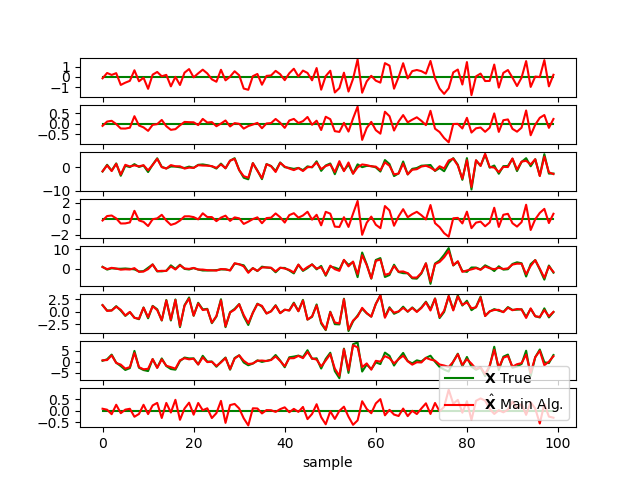
\includegraphics[scale=0.5]{figures/ch_estimate/k_test3.png}
	\caption{Each plot shows one row of the estimate $\hat{\mathbf{X}}_{\text{main}}$ using true $\mathbf{A}$, compared to the corresponding true row in $\mathbf{X}$. The MSE is $0.344$. Only samples in the interval $[0,100]$ are plotted.}
	\label{fig:ktest3}
\end{figure}
\noindent
It is expected that the precision must depend on the chosen tolerance for the mutual MSE. 
For comparison table \ref{tab:replica2}, \ref{tab:replica3} and \ref{tab:replica4} show the result from a tolerance of $0.5$, $1.5$ and $2$ respectively. 
It is observed that a tolerance of $0.5$ and $2$ results in a conclusion with respect to the number of zero rows -- being respectively 2 and 6. 
From this it is clear that the tolerance is difficult to define and will affect the conclusion of the results.  
\begin{table}[H]
\center
\begin{tabular}{|l|l|l|l|l|l|l|l|l|}
\hline
Row index   & 1 & 2 & 3 & 4 & 5 & 6 & 7 & 8 \\ \hline
\# replicas & 1 & 1 & 1 & 1 & 1 & 2 & 1 & 2 \\ \hline
\end{tabular}
\caption{Number of replicas for each row based on the tolerance MSE $< 0.5$.}
\label{tab:replica2}
\end{table}
\noindent
\begin{table}[H]
\center
\begin{tabular}{|l|l|l|l|l|l|l|l|l|}
\hline
Row index   & 1 & 2 & 3 & 4 & 5 & 6 & 7 & 8 \\ \hline
\# replicas & 1 & 4 & 1 & 3 & 1 & 4 & 1 & 3 \\ \hline
\end{tabular}
\caption{Number of replicas for each row based on the tolerance MSE $< 1.5$.}
\label{tab:replica3}
\end{table}
\noindent
\begin{table}[H]
\center
\begin{tabular}{|l|l|l|l|l|l|l|l|l|}
\hline
Row index   & 1 & 2 & 3 & 4 & 5 & 6 & 7 & 8 \\ \hline
\# replicas & 2 & 6 & 1 & 4 & 2 & 4 & 1 & 4 \\ \hline
\end{tabular}
\caption{Number of replicas for each row based on the tolerance MSE $< 2$.}
\label{tab:replica4}
\end{table}
\noindent
The results so far have relied on the true mixing matrix $\mathbf{A}$ as an input the main algorithm, due to the conclusion of chapter \ref{ch:implementation} where the estimate of $\mathbf{A}$ is abandoned. 
Thus, this gives the results to be expected conditioned on an exact estimate of $\mathbf{A}$ which this thesis does not manage to provide.

Now the investigations are repeated but with use of the main algorithm with a fixed $\mathbf{A}_{\text{fix}}$ provided as an input, cf. \ref{sec:test_base}.
Similar to figure \ref{fig:ktest3}, figure \ref{fig:ktest5} shows the estimates $\hat{\mathbf{X}}_{\text{main}}$ compared to the true $\mathbf{X}$. 
As expected, according to the results from section \ref{sec:Main_test}, it is generally seen from figure \ref{fig:ktest5} that every row of the estimate is less accurate as a result of using a fixed $\mathbf{A}_{\text{fix}}$ instead of the true $\mathbf{A}$. 
Table \ref{tab:replica5} shows the replica count with an MSE tolerance at 1. 
From the table it is seen that 7 out of the 8 rows are zero rows, while the true number is 4 rows. 
This could indicate that the tolerance is set to high. 
Table \ref{tab:replica6} show the replica count for an MSE tolerance at 0.5. 
From table \ref{tab:replica6} it is seen that the number of replicas is reduced.
However, it still does not result in the right number of zero rows.  
\begin{table}[H]
\center
\begin{tabular}{|l|l|l|l|l|l|l|l|l|}
\hline
Row index   & 1 & 2 & 3 & 4 & 5 & 6 & 7 & 8 \\ \hline
\# replicas & 3 & 5 & 2 & 2 & 4 & 1 & 4 & 5 \\ \hline
\end{tabular}
\caption{Number of replicas for each row based on the tolerance MSE $< 1$.}
\label{tab:replica5}
\end{table}
\noindent
\begin{table}[H]
\center
\begin{tabular}{|l|l|l|l|l|l|l|l|l|}
\hline
Row index   & 1 & 2 & 3 & 4 & 5 & 6 & 7 & 8 \\ \hline
\# replicas & 2 & 2 & 2 & 2 & 1 & 1 & 1 & 3 \\ \hline
\end{tabular}
\caption{Number of replicas for each row based on the tolerance MSE $< 0.5$.}
\label{tab:replica6}
\end{table}
\noindent
\begin{figure}[H]
\centering
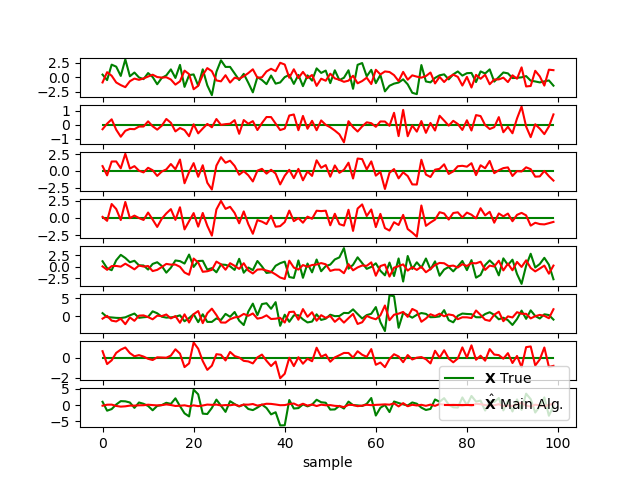
\includegraphics[scale=0.5]{figures/ch_estimate/k_test5.png}
\caption{Each plot shows one row of the estimate $\hat{\mathbf{X}}_{\text{main}}$ using $\mathbf{A}_{\text{norm2}}$, compared to the corresponding true row in $\mathbf{X}$. The MSE is $128.7$. Only samples in the interval $[0,100]$ are plotted.}
\label{fig:ktest5}
\end{figure}
\noindent
From the observations made through this investigation, based on synthetic data, the following conclusions are made.
From figure \ref{fig:ktest3} and table \ref{tab:replica1} a potential is found with respect to identifying the zero rows within the estimate. 
Here the zero rows are identified as the rows of the estimate for which similar signals appear in other rows indicating that no new estimate has been computed. 
From figure \ref{fig:ktest5}and table \ref{tab:replica5} and \ref{tab:replica6} a fixed $\mathbf{A}_{\text{fix}}$ is used in the main algorithm, as it will be when applied to real EEG data. 
Here it has not been possible to identify the zero rows correctly, based on the replica count. 
Thus, it must be concluded that the method is not reliable when the estimated is computed by the main algorithm. 
However, it is essential that a potential was found under ideal conditions, due to the results from the main algorithm being reliable as concluded in chapter \ref{ch:implementation}. 

However, to finish the investigation, the method replica count has been applied to the estimation of real EEG data. This is done due to the possibility of seen a different behavior from the real EEG data compared to the synthetic data. 

\section{Empirical Test on EEG Measurements}
Consider now the same estimation of the number of active sources, $k$, but from the real EEG measurements. 
For this estimation one can not compare the estimation to the real sources as in the previous section.
Hence, the replica count method is just applied an estimation $\hat{\mathbf{X}}_{\text{main}}$ of real EEG measurements and a conclusion is made from the observed result.

The source signal estimation is performed on segment 10 from the \texttt{S1\_Cclean} EEG data set, where every second sensor is removed to achieve the case where $M < N$. 
Specifically $\hat{\mathbf{X}}_{\text{main}}$ is computed given $k = N$ and $\hat{\textbf{A}}_{\text{fix}}$ resulting from segment of EEG measurements specified by $M = 1/2 N = 13$. 

Figure \ref{fig:eeg_k} visualize the recovered source matrix $\hat{\mathbf{X}}_{\text{main}}$ from time segment $s = 10$ for $M = 13$ and $k = N = 27$. For visual simplicity only 8 out of 27 sources are visualized.
\begin{figure}[H]
    \centering
	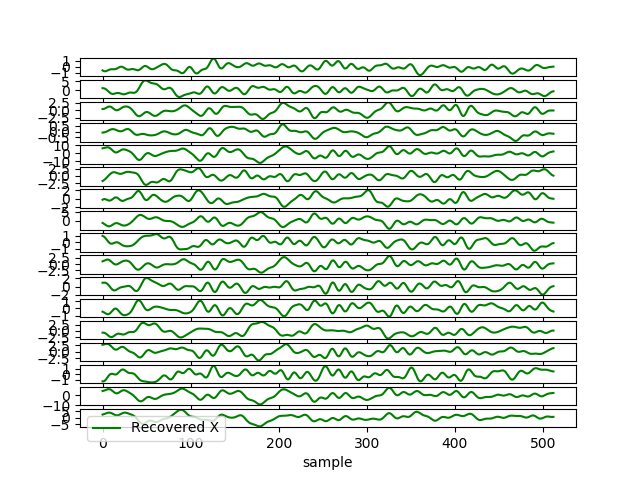
\includegraphics[scale=0.5]{figures/ch_estimate/eeg_k_timeseg_10.png}
	\caption{The recovered source matrix $\hat{\mathbf{X}}_{\text{main}}$ from time segment $s = 10$ from \texttt{S1\_Cclean} for $M = 13$ and $k = N = 27$. Note only the first 8 rows of $\hat{\mathbf{X}}_{\text{main}}$ is plotted for simplicity.}
	\label{fig:eeg_k}
\end{figure}
\noindent
From figure \ref{fig:eeg_k} it is seen that all $10$ source signals appears to be active -- the non visualized source signals do also appears to be active.
Furthermore, there seem not to be any visible indication of an active source being non-active, with respect to being a direct replica. 

By applying the replica count method to $\hat{\mathbf{X}}_{\text{main}}$  from figure \ref{fig:eeg_k} only one source signal is not considered replicas. 
This potentially active source signal is found in row 13, the last row plot on figure \ref{fig:eeg_k}. 
This leads to the conclusion that for time segment $s = 10$ with system specification $M = 13$ for the \texttt{S1\_Cclean} EEG data set only have $k = 1$ active sources. 



